\documentclass[twoside]{article}

\usepackage[math]{kurier}
\usepackage[sc]{mathpazo}
\usepackage{outlines}
\usepackage{hyperref}
\renewcommand{\sfdefault}{kurier}

\usepackage{framed} % or, "mdframed"
\usepackage[framed]{ntheorem}
\newframedtheorem{frm-def}{Definition}

\hypersetup{
  colorlinks   = true,    % Colours links instead of ugly boxes
  urlcolor     = blue,    % Colour for external hyperlinks
  linkcolor    = blue,    % Colour of internal links
  citecolor    = red      % Colour of citations
}

\usepackage{graphicx}
\setlength{\oddsidemargin}{0.25 in}
\setlength{\evensidemargin}{-0.25 in}
\setlength{\topmargin}{-0.6 in}
\setlength{\textwidth}{6.5 in}
\setlength{\textheight}{8.5 in}
\setlength{\headsep}{0.75 in}
\setlength{\parindent}{0 in}
\setlength{\parskip}{0.1 in}

\usepackage{listings}
\usepackage{color}
\definecolor{mygreen}{rgb}{0,0.6,0}
\definecolor{mygray}{rgb}{0.5,0.5,0.5}
\definecolor{mymauve}{rgb}{0.58,0,0.82}

\lstset{ %
  columns=flexible,
  backgroundcolor=\color{white},   % choose the background color
  %basicstyle=   % size of fonts used for the code
  breaklines=true,                 % automatic line breaking only at whitespace
  captionpos=b,                    % sets the caption-position to bottom
  commentstyle=\color{mygreen},    % comment style
  escapechar=\%*,          % if you want to add LaTeX within your code
  keywordstyle=\color{blue},       % keyword style
  stringstyle=\color{mymauve},     % string literal style
}

\usepackage{hyperref}
\hypersetup{
    colorlinks=true,
    linkcolor=blue,
    filecolor=magenta,      
    urlcolor=cyan,
}
 
\urlstyle{same}
 


\newcounter{lecnum}
\renewcommand{\thepage}{\thelecnum-\arabic{page}}
\renewcommand{\thesection}{\thelecnum.\arabic{section}}
\renewcommand{\theequation}{\thelecnum.\arabic{equation}}
\renewcommand{\thefigure}{\thelecnum.\arabic{figure}}
\renewcommand{\thetable}{\thelecnum.\arabic{table}}


\newcommand{\lecture}[4]{
   \pagestyle{myheadings}
   \thispagestyle{plain}
   \newpage
   \setcounter{lecnum}{#1}
   \setcounter{page}{1}
   \noindent
   \begin{center}
   \framebox{
      \vbox{\vspace{2mm}
    \hbox to 6.28in { {\bf \sffamily AA 274: Introduction to Robotic Autonomy
                        \hfill Winter 2019} }
       \vspace{4mm}
       \hbox to 6.28in { {\sffamily{\Large \hfill Lecture #1 #2  \hfill}} }
       \vspace{2mm}
       %\hbox to 6.28in { {\it \hfill Scribes: #4} }
      \vspace{2mm}}
   }
   \end{center}
   \markboth{Lecture #1: #2}{Lecture #1: #2}

   \vspace*{4mm}
}



%%%%%%%%%%%%%%%%%%%%%%%%%%
%document
\begin{document}
%modify this
\lecture{2}{The Robot Operating System (ROS)}{}

\section{Introduction}\label{intro}
Experts in the Silicon Valley have said that we now live in a Golden Age of robotics, where high-quality hardware is both affordable and easily accessible. The developments of the past decade have enabled professionals and hobbyists alike to develop robotics from the comfort of their homes. This growth in the robotics industry is fortuitously bolstered by the existence of the Robot Operating System (ROS), a robust robotic development platform that will be introduced in this lecture.

We will first look at brief history of ROS (Section \ref{history}), which will shed some light on motivation to develop a brand new robotics development platform from scratch, as well as its core values (Section \ref{characteristics}). Next we will look into the building blocks of ROS, namely the nodes, the master and the message types in ROS  (Section \ref{main_component}). Based on the comprehensive understanding of the skeleton of ROS, we will work a few examples with ROS that will give even more insights on the workings of ROS (Section \ref{programming}). Specifically, in our first example we will see interactions among different nodes by creating a publisher and a subscriber of example messages. Our second example will show how a simple ROS codes can easily integrate to an external framework (USB-operated camera) seamlessly (Section \ref{programming}). At the end of this chapter, we will explore Catkin, a build system for ROS to manage several components of ROS that can make ROS management much easier(Section \ref{development}). 

%\subsection{Outline and Learning Objectives}

\begin{outline}
    \footnotesize
    \1 \hyperref[sec:history]{A Brief History of ROS}%: Learn the motivations behind the development of ROS as a robotics development platform.
    \1 \hyperref[sec:characteristics]{Characteristics of ROS}%: Learn how ROS integrates with existing software/hardware using the Publish-Subscribe (Pub/Sub) Model, along with alternative communication models.
    \1 \hyperref[sec:maincomponent]{Main Components of ROS}%: Learn more about the Pub/Sub model, as well as its three main components: the Nodes, the Master, and the Message Types.
    \1 \hyperref[sec:programming]{Basic of Programming with ROS}%: Learn how to create both publisher and subscriber nodes, run nodes, monitor messages, as well as launch files.
    \2 Creating a Publisher
    \2 Running the Node and Monitoring Messages
    \2 Creating a Subscriber
    \2 Launch Files
    \2 Case Study using a USB Camera
    \1 \hyperref[sec:development]{Developing with ROS}%: Learn to
    \2 Catkin and ROS Packages
    \2 Debugging
    \2 Useful Message Types
    \3 Diagnostic Messages
    \3 Navigation Messages
    \3 Geometry Messages
    \3 Sensor Messages
    \3 Built-in Message Types
    \2 Useful Features
    \1 \hyperref[sec:help]{Getting Help}
    \1 \hyperref[sec:bib]{References and Further Reading}
\end{outline}


\section{Brief History of ROS}\label{history}\label{sec:history}
Until the advent of ROS, there existed no way for various robotics developers to collaborate or share work among different teams, projects or platforms. In 2007, earliest versions of ROS start to be conceived at Stanford AI Robot (STAIR) project with the following vision:

\begin{itemize}
    \item The new robotics development environment should be free and open-source for everyone, and need to remain so. This environment will encourage (and live off of) collaboration of community members.
    \item The new platform should make core components of robotics --from its hardware to library packages  -- readily available for anyone who intend to launch a robotics project.
    \item The new software development platform should integrate a number of existing framekworks that were targeted at specific aspects of robotics (OpenCV, SLAM, Gazebo, etc)
\end{itemize}

Development of ROS started to gain tangible traction when Scott Hassan, a software architect and entrepreneur, founded a startup called Willow Garage to develop standardized robotics development platform in Menlo Park. 

While mostly self-funded by the founder Scott Hassan himself due to its open-source nature, Willow Garage proved to have perfectly met the dire needs to build a standardized development environment for robotics projects. PR2 (Figure 2.1) was one of earliest humanoid robot on wheels that expedited development of ROS, which were awarded to 11 universities across the country for further collaboration on ROS development. 
Starting 2012, Open Source Robotics Foundation (OSRF) supervises the future of ROS by supporting development, distribution, and adoption of open software and hardware for use in robotics research, education, and product development. As of this day, ROS is 11yrs old and still maintained by the OSRF along with Gazebo, a virtual robotic simulator.
\begin{figure}[ht]\label{fig:1}
\centering
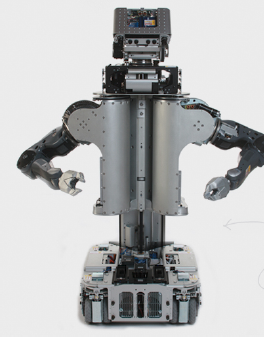
\includegraphics[width=0.5\textwidth]{PR2}
\caption{Overview of a PR2 robot}
\end{figure}

\section{Characteristics of ROS}\label{characteristics}\label{sec:characteristics}
%Talk about:
%-integration with existing framework (either etalk about it here, or just lump it together to 'core values of ROS')
%-modularity
%-sub/pub
Despite what its name suggests, ROS is a middleware or framework rather than an operating system. The Robot Operating System can be described as a collection of tools, libraries, and conventions that aim to simplify the task of creating complex and robust robot behavior across a wide variety of platforms. At its creation, it was the integration of many existing projects and specific ecosystems, such as OpenCV (computer vision), Stage (2D simulator), Gazebo (3D simulator), OpenSLAM (navigation), Orocos KDL (arm navigation), and other ROS wrappers. Integrating ROS in one's project seldom takes more than a couple of lines of code; it can be seen simply as "gluing" components to work together. The development is mostly in languages such as Python or C++.

Although many of today's robotic platforms did not exist when Willow Garage was coming up with ROS, the developers were visionary enough to design the software to be compatible with any general robot - whether it be a flying quadcopter, a wheeled rover, or a bipedal humanoid. Early ROS developers learned that a powerful and efficient method to handle the complexity of robotic software could be accomplished using modules, as shown in Figure 2.2. This modularity takes the form of independent robotic components that perform separate functions and simplify the exchange of information. These components, called "nodes", share data with one another and act as the basic building blocks of ROS. Nodes can vary in function from sensor drivers at the low-level to even high-level tasks such as path planning with dynamic obstacle avoidance. Processing big data among nodes may cause CPU or GPU to be overwhelmed. To reduce computation on local computers, ROS is designed to be a network-aware application. To be specific, the software design pattern used to facilitate the message exchange between nodes is known as the Publish-Subscribe (Pub/Sub) model. Publishing means to send messages no matter whether there are listeners. Subscribing is to receive messages as long as there is a publisher. There are some alternatives to the Pub/Sub model, such as Request/Reply, Push/Pull, data binding, and observers. As far as within the context of this course, Pub/Sub is the communication framework that ROS relies on.

Many other frameworks were created as "alternatives" of ROS. Some of these frameworks are Lightweight Communications and Marshalling (LCM), Drake, Player, YARP, Orocos, and MRPT. Despite the existance of other frameworks, ROS is the one closest to the industry standard. Meanwhile, it possesses the higher stability and various online resourses as described below. Thus, ROS is the choice in AA274. 
\begin{figure}[ht]
\centering
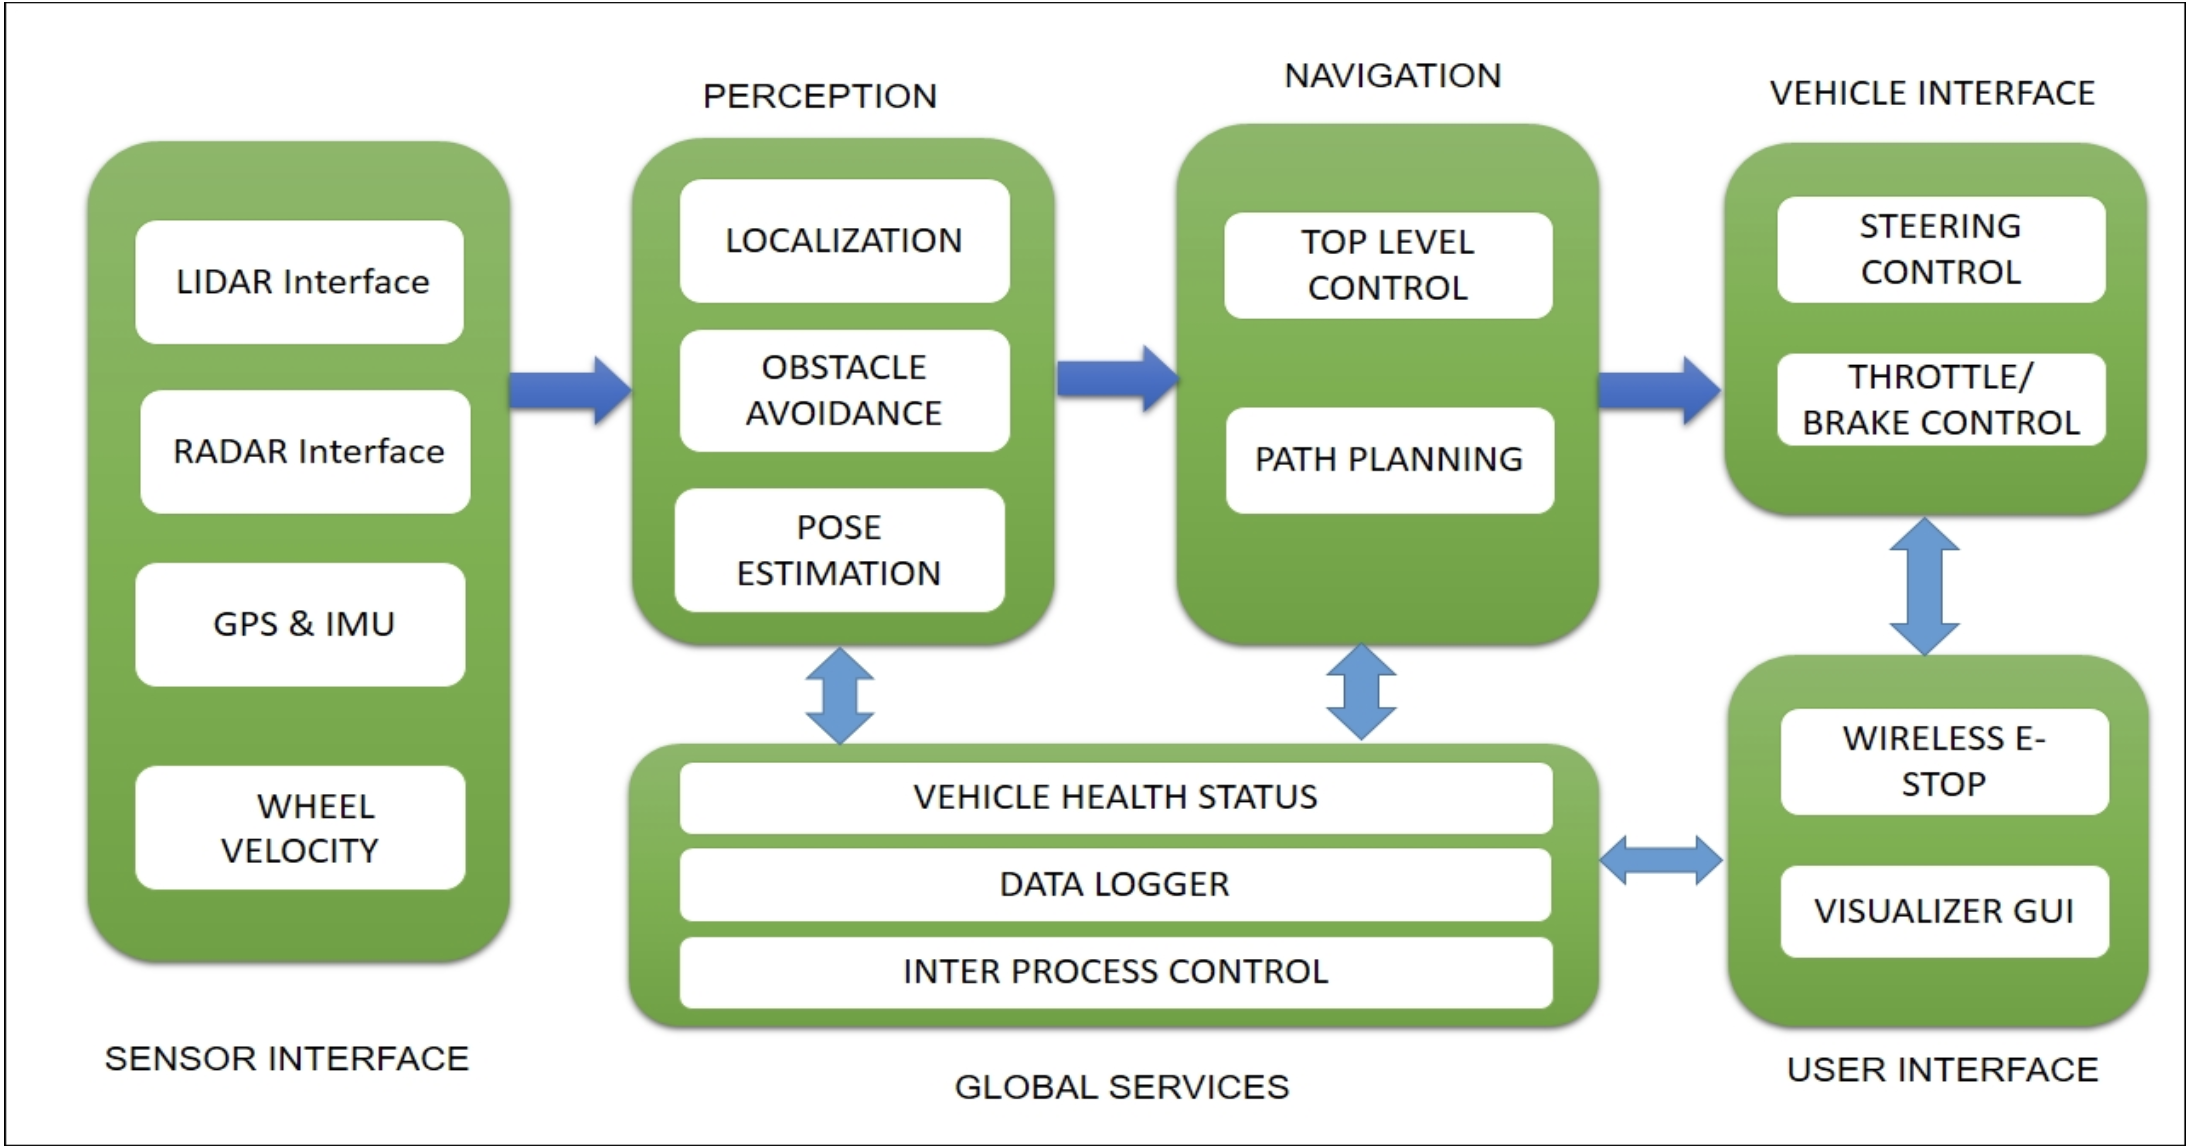
\includegraphics[width=1\textwidth]{ModularityPhoto}
\caption{Modularity designed for the complexity of robotic programming.}
\end{figure}

\section{Main Components of ROS} \label{main_component}\label{sec:maincomponent}
The three main components of ROS with the Pub/Sub programming model are the Nodes, the Master, and the Message Types. The nodes are responsible for publishing or subscribing to certain pieces of information that are shared within a virtual "chat room" called a topic. The publisher and subscriber nodes communicate with each other via these topics to perform their functions. A separate software called the master is a process that can run on any piece of hardware to coordinate the exchange between the publishers and subscribers. It is responsible for assigning network addresses to ensure that publishers and subscribers are connected to the correct topics, even if they are running on different computers. The information is securely exchanged using message types, which serve as a powerful abstraction away from specific pieces of hardware. Using message types, nodes can read certain data types (i.e. camera image, laser scan data, motion control) in the same way regardless of hardware brand or design. For instance, a LiDAR node and a mobile robot controller publishes laser scan arrays and odometry values respectively in two sensor message types. By subscribing these message types, a navigation node can receive the message sent from the sensors and send out corresponding motion control messages. 

\begin{frm-def}[Master]
The master is a process that is in charge of coordinating nodes, publishers, and subscribers. There is exactly one running at any time. The master allows the nodes to find each other but is not used to send or receive messages.
\end{frm-def}

A unique feature of the master process is that is does not need to exist within the robot's hardware. The master can be facilitated remotely, on a much larger and more powerful computer and its execution is not constrained by the robotic components. Furthermore, the messages published within the topics do not go through the master; the exchange is peer-to-peer between the nodes.\\ % Add more stuff about master here.

\begin{frm-def}[Node]
A node is a process that is connected to the Pub/Sub network in ROS. Nodes communicate with each other via topics to perform tasks.
\end{frm-def}

Any system built using ROS consists of nodes, which are small parts of the larger program that work together to form a robot system. Nodes can be sensors, actuators, or simply computations that work in tandem with one another. For example, a simple system might consist of a distance sensor and a motor on a wheeled robot. If the robot wants to be some distance from a wall, the distance sensor node detects the current position and sends that information to the motor node, which acts to move the robot toward the desired position. There is no great reason that a system like that needs nodes, but suppose now the robot wants to stay centered between two walls. Adding a new sensor node for a second distance sensor is somewhat trivial. This can be further expanded to add more sensors and actuators. The node system allows the user to scale up to very complex robots by adding nodes for each additional component.\\

\begin{frm-def}[Message]
Nodes communicate with each other via peer-to-peer messages. Some common message types are camera images, laser scan data, and motion control commands.
\end{frm-def}

The peer-to-peer message system that ROS uses is illustrated in Figure 2.3. Messages contain information such as sensor data and commands. The messages (Msg) are sent over a topic. For example, sensor nodes send messages to various topics, which controller nodes access to send commands to motors and actuators to move the robot or perform some other action.\\

\begin{figure}[ht]
\centering
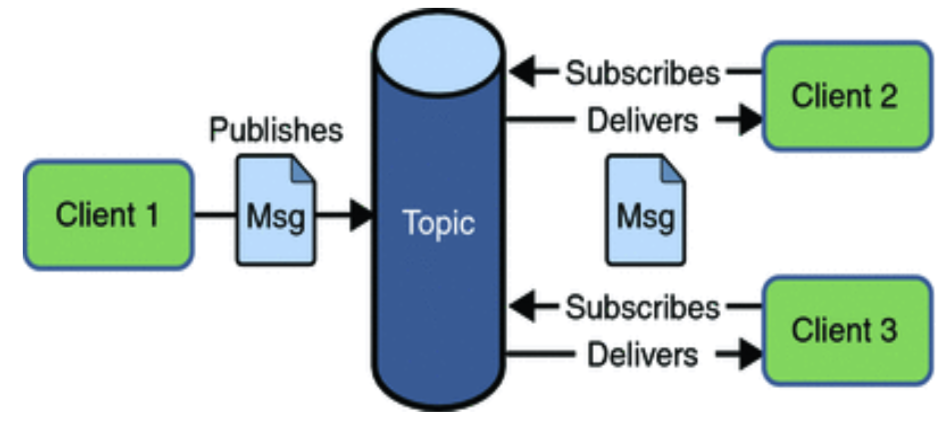
\includegraphics[width=0.7\textwidth]{ChatRoom}
\caption{The publish/subscribe model.}
\end{figure}

\begin{frm-def}[Topic]
In ROS, every message is sent using a topic. Some nodes send messages through the topic and other nodes receive messages through the topic. Topics are analogous to chat rooms.
\end{frm-def}

Topics are the medium in which nodes exchange messages in ROS. A node sends a message to a topic and any node that subscribes to that topic receives the message. In Figure 2.3, "Client 1" sends a message (publishes) to the topic and since both "Client 2" and "Client 3" listen (subscribe) to that topic, they will both receive the message. In ROS, these "clients" are nodes.

{\it Note: Topics can have any number of publishers and subscribers. Typically, having multiple publishers on a topic is a mistake.} \\

\begin{frm-def}[Publisher]
A publisher is a node that sends messages through a topic.
\end{frm-def}

Publishers are nodes that "publish" messages to a topic for other nodes to receive. These publisher nodes could be sensors that are transmitting data such as force or temperature. They might also be a controller sending out commands to control the motion of the robot. The publisher sends its messages with no regard for what nodes, if any, are looking for the message. Referring again to Figure 2.3, "Client 1" is the publisher.

{\it Note: If no nodes are subscribed to a published message, ROS automatically does not publish the unused data to preserve bandwidth.} \\

\begin{frm-def}[Subscriber]
A subscriber is a node that receives messages through a topic.
\end{frm-def}

When sensors or other publishers send their messages, there must be nodes to receive them. These nodes are called subscribers. They "subscribe" to a topic to receive relevant information in order to perform a task. For example, these subscribers might collect information from sensors to determine location or pass commands to control actuators. In Figure 2.3, "Client 2" and "Client 3" are subscribers receiving messages from the topic.\\

\section{Basics of programming with ROS}\label{programming}\label{sec:programming}
\subsection{Creating a Publisher}
Starting a publisher consists of creating a node, setting a topic name, defining the type of message that will be sent, and setting a rate at which to send the message and a queue size for held messages. Nodes must have unique names; specifying the 'anonymous' option in node initialization allows the use of identical copies of a node, adding anonymous appendages to their names for uniqueness.
Sample code for creating a publisher node named "talker" is given below. The topic is "chatter" and it sends a string once per second.

\begin{lstlisting}[language=python]
import rospy
from std_msgs.msg import String
#std_msgs contain wrappers for ROS primitive types documented %*\href{http://wiki.ros.org/std_msgs}{here}%*. 
#String is one of the primitive types available.

def talker():
    rospy.init_node('talker', anonymous=True)
    #create a node. 'talker' is the node name.
    #The anonymous=true setting allows the master to check whether that name exists
    #already on the network and appends characters to make the name unique.
    #This is useful if you don't care about unique name for tools or GUIs, 
    #but unique names (anonymous=False) are important for nodes like drivers.

    pub.rospy.Publisher('chatter', String, queue_size=10)
    #chatter is the topic name, the message type is a string,
    #and there can be 10 messages in the queue. It is recommended that
    #you have a queue size at least equal to the publish rate to avoid missed messages.

    rate = rospy.Rate(1)
    #sets the rate to 1 Hz. A message will be sent approximately once per second

    rospy.loginfo("Starting ROS node talker...")
    #this message sends when the publisher node starts up

    while not rospy.is_shutdown(): #as long as ROS is still running
        msg = "Greetings humans!" #define a message to send
        pub.publish(msg) #send the message
        rate.sleep() #wait until it is time to go again, defined by rate

if __name__ == '__main__':
    try:
        talker() #run the above function
    except rospy.ROSInterruptException: #if there is an error
        pass #this ignores the error. Often something else would be here

\end{lstlisting}

Another option available when creating a publisher is the "latch." This allows a new subscriber to receive the last message sent. It can be useful for messages that are only sent once or very infrequently to allow new subscribers to receive the message without waiting for another update.

\subsection{Running the Node and Monitoring Messages}
% I think a section on how to get information from the command line might be useful. Things like the subscriber thing shown in lecture
% going to get the stuff from the video tomorrow (Sunday) and fill this in - Patrick
% re-arranged section headings around a bit and so added to this sub-section: let me know how this reads/ feel free to edit - Dipti
% I think command line things should come after we introduce the components, like it was before
The command 'rosrun' can be used to fire up this publisher node by specifying its name and the package it belongs to (more on packages later): for instance,
\begin{verbatim}
	rosrun aa274 talker.py
\end{verbatim}
As noted above, however, a publisher does not send messages until the topic is actually subscribed to. The rostopic command line tool offers a handy way to subscribe to a topic to monitor its messages. Below we list three most common rostopic commands:\\ \\
{\ttfamily
\begin{tabular}{l l}
rostopic list & lists all active topics \\
rostopic echo $<topic>$ & prints messages received on topic \\
rostopic hz $<topic>$ & measures topic publishing rate \\
\end{tabular}
}

The last command is particularly useful in debugging responsiveness of an application, for example in the face of a lossy connection in deep learning vision work.

\subsection{Creating a Subscriber}
Much like the publisher definition above, A subscriber node needs a subscriber function, specifying the topic name, message type, and a handle to a callback function. This callback function takes the incoming message as a parameter and performs some operation, such as printing the message data. The sample program below creates a subscriber node 'listener' that subscribes to the 'chatter' topic published by the 'talker' node.
\begin{lstlisting}[language=python]
import rospy
from std_msgs.msg import String

def callback(msg):
    rospy.loginfo("Received: %s", msg.data)
    #record the message as received
    #callback is the section where you specify commands based on messages received
    #You can multiple callback and listener function in the same .py file

def listener():
    rospy.init_node('listener', anonymous=True)
    #create a node. 'listener' is the node name.
    #The anonymous setting allows the master to append characters to make the name unique.

    rospy.Subscriber("chatter", String, callback)
    #subscribe to the "chatter" topic, receiving Strings.
    #callback is filled by the above function

    rospy.loginfo("Listening on the chatter topic...")
    #indicate that the subscriber has started

    rospy.spin()
    #keep listening for messages

if __name__ == '__main__':
	listener()
\end{lstlisting}

\subsection{Launch Files}
The launch file can be seen as the ROS notion of an application: instead of separately launching each subscriber and publisher node, ROS programmers can create Extensible Markup Language (XML) launch files to simultaneously start the master, execute multiple nodes, and set node parameters in a single executable. A simple example is given below. It starts with a comment to describe the file. Then, it creates a node with the name "talker" in the package "aa274" that outputs to the screen 5 times per second.
\begin{lstlisting}[language=XML]
<launch>
    <!-- Start the talker node -->
    <node name="talker" pkg="aa274" type="talker.py" output="screen">
        <param name="rate" value="5"/>
        <!--Note: talker.py must be executible or ROS will not find it-->
    </node>
</launch>
\end{lstlisting}

\subsection{Case Study using USB Camera}
An example of a more complex application of ROS is shown in class through the case study of edge detection in a camera image. A camera node connects to a USB camera, publishing raw images. An edge detection node runs on these raw images and publishes its processed images. Image view nodes subscribe to and display both images. A single launch file, shown below, launches all the nodes. An rqt\verb|_|graph, shown in Figure 2.4, helps visualize the connections between various publishers and subscribers. This case study demonstrates how a complex function can be accomplished simply by launching pre-existing nodes in ROS.

The four nodes used in this edge detection example are summarized below in more detail, indicating the name of the node as shown in the rqt\verb|_|graph, anything the node subscribes to, and anything the node publishes:

\textbf{Node 1 --– Camera Driver} $\rightarrow$ \textit{subscribes to: nothing, publishes: camera images.}
\\
\textbf{Node 2 --– Edge Detection} $\rightarrow$ \textit{subscribes to: camera images, publishes: image with edges.}
\\
\textbf{Node 3 --– image\_view} $\rightarrow$ \textit{subscribes to: camera images, publishes: nothing.}
\\
\textbf{Node 4 --– image\_view} $\rightarrow$ \textit{subscribes to: image with edges, publishes: nothing.}



\begin{lstlisting}[language=XML]
<launch>
    <arg name="video_device" default="/dev/video0" />
   
    <!-- Launch USB cam driver -->
    <include file="$(find aa274)/launch/usbcam_driver.launch">
        <arg name="video_device" value="$(arg video_device)" />
    </include>
   
    <!-- Create node to subscribe to colour image topic and view
    raw camera image in a window -->
    <node name="image_view_1" pkg="image_view" type="image_view">
        <remap from="image" to="/camera/image_color" />
        <param name="autosize" value="true"/>
    </node>
    
    <!-- Create node to process output of edge detection node
    and view resultant image in a window -->
    <node name="image_view_2" pkg="image_view" type="image_view">
        <remap from="image" to="/edge_detection/image" />
        <param name="autosize" value="true" />
    </node>

    <!-- Create an open CV package based node to subscribe to colour image
    topic and run edge detection function on the subscribed images-->
    <node name="edge_detection" pkg="opencv_apps" type="edge_detection">
        <remap from="image" to="/camera/image_color" />
        <param name="debug_view" value="false" />
    </node>
</launch>
\end{lstlisting}

\begin{figure}[ht]
\centering
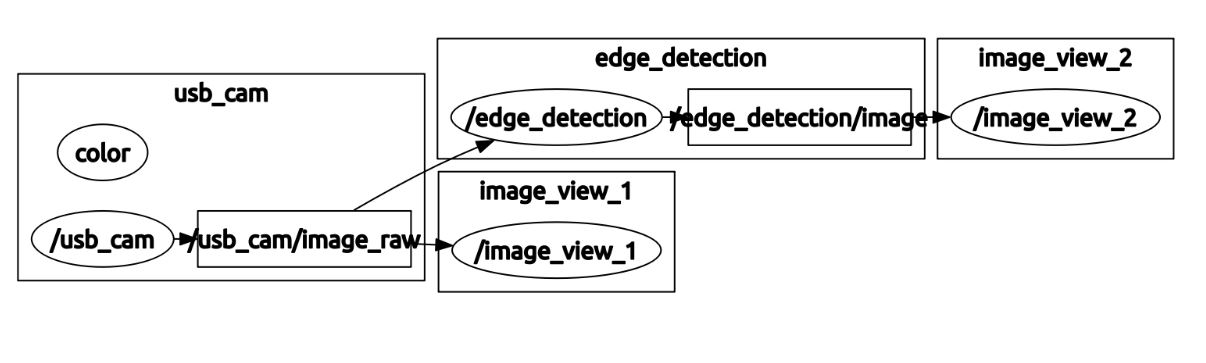
\includegraphics[width=1\textwidth]{USBCamera}
\caption{rqt graph of the edge detection case study.}
\end{figure}

Beyond edge detection, the ROS package "opencv\_apps" contains a multitude of computer vision functionalities that can be easily incorporated as ROS nodes. These rigorously developed computer vision algorithms include bounding box generation, face and body detection, motion analysis, and image filters. The ROS Wikipedia page provides extensive documentation for the "opencv\_apps" package, including detailed descriptions of each algorithm, explanations of parameters, and visual examples demonstrating many of the algorithms. One can also contribute to the computer vision package -- and any other ROS source code -- by editing or adding to the Github repository for this package.

\section{Developing with ROS}\label{development}\label{sec:development}
\subsection{Catkin and ROS Packages}
Catkin is a build system for ROS and a Catkin workspace can be used to organize python scripts, launch files, etc in the form of nodes and packages. It's built on top of CMake, with additional features to tackle the complex dependencies that arise with ROS. ROS Packages are collections of nodes usually corresponding to a functionality, e.g. SLAM, and serve as the basic organizational structure for nodes.
Initializing a Catkin workspace allows one to manage the building of packages in its src directory:

\begin{verbatim}
mkdir -p ~/catkin_ws/src
cd ~/catkin_ws
catkin_make
\end{verbatim}

When a Catkin package is created, it is initialized with a CMakeLists file and a package.xml. Besides these, one typically needs sub-folders for config files, launch files and scripts as shown in Figure 2.4. Additional sub-folders may be required for more complex packages.
\begin{figure}[ht]
\centering
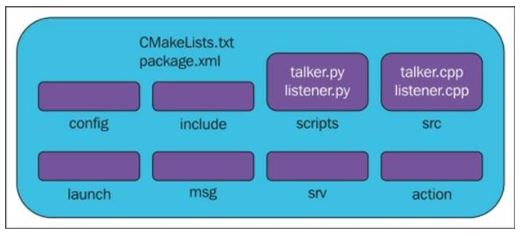
\includegraphics[width=0.8\textwidth]{ROSPackage}
\caption{The components of a typical ROS package in a Catkin workspace.}
\end{figure}

\subsection{Debugging}
Just as \verb|rostopic| enables us to monitor ROS topics in the command line, \verb|rospy.loginfo()| starts a background process that writes ROS messages to a ROS logger, viewable through a program such as \verb|rqt_console.|
Similarly, \verb|rosbag| provides a convenient way to record a number of topics for playback.

\subsection{Useful Message Types}
ROS messages are data structures which contain information that is to be sent from one node to another. The type of a message is important as a publisher and subscriber must send and receive the same type in order to communicate. Therefore, a topic type is defined by the type of the message being published to the topic. The command \texttt{rostopic type [topic]} can be used to view the type of message being published to a topic. A msg file contains the field type and the corresponding field name. The field type refers to the message type, which defines the type of information it stores. The field name simply refers to the name of the message, which usually indicates the data being sent. Empty brackets \texttt{[]} can be appended to the field name to indicate that it is an array of that type.

A msg file has the following structure: field type, field name

An example is:
\begin{verbatim}
myp_ros/msg/SensorPacket.msg 
time            stamp
SensorData[]    sensors
uint32          length
\end{verbatim}

In the following sections a few examples of message types belonging to common categories will be discussed. These categories are divided into diagnostic, navigation, geometry and sensor messages. These are just a selection of messages frequently used by other ROS packages, for a more comprehensive list refer to the \texttt{common$\_$msgs} documentation.


\subsubsection{Diagnostic Messages} 
\textbf{GoalStatus}\newline
Returns an integer indicating the status of a goal. Message can be adjusted to contain and send a number of goals using an array form of the message. Nine possible states; PENDING=0, ACTIVE=1, ... , RECALLED=8, LOST=9.
\begin{verbatim}
uint8, status  
\end{verbatim}
%\vspace{-9pt}

\textbf{DiagnosticStatus} \newline
Message returns the status of a component within the robot, Possible states; OK=0, WARN=1, ERROR=2 and STALE=3. This message can also be extended to return the status of multiple components using an array version of the message.
\begin{verbatim}
byte level # level of operation 
string name # a description of the test/component reporting
string message # a description of the status
string hardware_id # a hardware unique string
KeyValue[] values # an array of values associated with the status
\end{verbatim} 

\textbf{KeyValue} \newline
Used to track a value over time, during simulation. 
\begin{verbatim}
string key # what to label the value when viewing
string value # value to track over time
\end{verbatim}

\subsubsection{Navigation Messages}

\textbf{GridCells} \\
An array of cells in a 2D grid.
\begin{verbatim}
Header header
float32 cell_width
float32 cell_height
geometry_msgs/Point[] cells
\end{verbatim}

\textbf{OccupancyGrid} \\
This represents a 2-D grid map, in which each cell represents the probability of occupancy. The third line describes the map data, in row-major order, starting with (0,0). Occupancy probabilities are in the range [0,100]. Unknown is -1.
\begin{verbatim}
Header header 
MapMetaData info
int8[] data
\end{verbatim}

\textbf{Path} \\
An array of poses that represents a Path for a robot to follow.
\begin{verbatim}
Header header
geometry_msgs/PoseStamped[] poses
\end{verbatim}

\subsubsection{Geometry Messages}

\textbf{Pose} \\
A representation of pose in free space, composed of position and orientation.
\begin{verbatim}
Point position
Quaternion orientation
\end{verbatim}

\textbf{Point} \\
This contains the position of a point in free space.
\begin{verbatim}
float64 x
float64 y
float64 z
\end{verbatim}

\textbf{Quaternion} \\
This represents an orientation in free space in quaternion form.
\begin{verbatim}
float64 x
float64 y
float64 z
float64 w
\end{verbatim}

\subsubsection{Sensor Messages}

\textbf{CompressedImage} \\
This message contains a compressed image. The header timestamp should be acquisition time of image. The header frame\_id should be optical frame of camera. The origin of frame should be optical center of camera. The +x should point to the right in the image, +y should point down in the image and +z should point into to plane of the image. The format should be specified as either jpeg or png. The third line is the compressed image buffer.
\begin{verbatim}
Header header
string format
uint8[] data
\end{verbatim}

\textbf{Imu} \\
This is a message to hold data from an IMU (Inertial Measurement Unit). Accelerations should be in $m/s^2$, and rotational velocity should be in rad/sec.

\begin{verbatim}
Header header
geometry_msgs/Quaternion orientation
float64[9] orientation_covariance
geometry_msgs/Vector3 angular_velocity
float64[9] angular_velocity_covariance
geometry_msgs/Vector3 linear_acceleration
float64[9] linear_acceleration_covariance
\end{verbatim}

\textbf{PointCloud} \\
This message holds a collection of 3d points, plus optional additional information about each point. The header specifies the the time of sensor data acquisition and coordinate frame ID. The second line is an array of 3d points. Each Point32 should be interpreted as a 3d point in the frame given in the header. For the third line, each channel should have the same number of elements as points array, and the data in each channel should correspond 1:1 with each point. Channel names in common practice are listed in ChannelFloat32.msg.
\begin{verbatim}
Header header
geometry_msgs/Point32[] points
ChannelFloat32[] channels
\end{verbatim}

\subsubsection{Built-in Message Types}
%%https://github.com/fp-robotics/myp_ros/wiki/Messages-and-Topics:-Communicating-between-nodes
The available built-in message types available in ROS are listed below in Table \ref{table:Built-in Messages}. The first column contains the message type, the second column contains the serialization type of the data in the message and the third column contains the numeric type of the message in Python.
\begin{table}[h]
\centering
\begin{tabular}{lll}
\hline
\textbf{Primitive Type} & \textbf{Serialization}          & \textbf{Python} \\ \hline
bool (1)                & unsigned 8-bit int              & bool            \\
int8                    & signed 8-bit int                & int             \\
uint8                   & unsigned 8-bit int              & int (3)         \\
int16                   & signed 16-bit int               & int             \\
uint16                  & unsigned 16-bit int             & int             \\
int32                   & signed 32-bit int               & int             \\
uint32                  & unsigned 32-bit int             & int             \\
int64                   & signed 64-bit int               & long            \\
uint64                  & unsigned 64-bit int             & long            \\
float32                 & 32-bit IEEE float               & float           \\
float64                 & 64-bit IEEE float               & float           \\
string                  & ascii string (4)                & str             \\
time                    & secs/nsecs unsigned 32-bit ints & rospy.Time      \\ \hline
\end{tabular}
\caption{Built-in Messages} \label{table:Built-in Messages}
\end{table}

\subsection{Useful Features}
Custom Messages, ROS Services, Parameter Server and Dynamic Reconfigure are a few other useful features offered by ROS. ROS uses the Universal Robot Description Format (URDF) to specify the kinematic chain of robot models, allowing it to compute coordinate transforms between their different components. Gazebo is a (mostly) accurate physics simulator that is useful for testing code on a virtual robot, as shown in Figure 2.6.
\begin{figure}[ht]
\centering
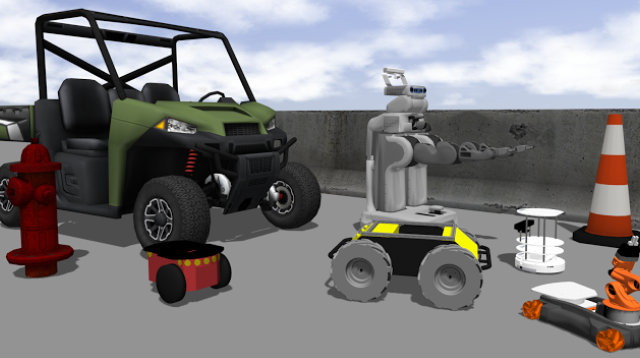
\includegraphics[width=0.7\textwidth]{Gazebo}
\caption{Screenshot of a Scene in Gazebo}
\end{figure}

\newpage
\section{Getting Help}\label{sec:help}

There are many resources at your disposal for getting help with ROS. The following resources were mentioned in the slide-deck of this lecture:

\begin{itemize}
\item \textbf{ROS wiki} (\url{http://wiki.ros.org/})
\newline
The ROS wiki is the official documentaion for ROS and is often the best source. In addition, on the ROS wiki there is a question and answer forum if you cannot find what you need in the documentation (\url{https://answers.ros.org/questions/}). Turtlesim on the ROS wiki provides a simple lightweight  simulation environment to learn ROS basics (\url{http://wiki.ros.org/turtlesim}).

\item \textbf{General References and Forums}
\newline
GitHub, Stack Overflow, Youtube and Google
\item \textbf{The Construct} (\href{https://www.youtube.com/channel/UCt6Lag-vv25fTX3e11mVY1Q}{link}) /\textbf{Robot Ignite Academy}(\url{http://www.theconstructsim.com})
\newline 
The Robot Ignite Academy is a paid resource that features interactive online classes using simulated robots. However, The Construct is their Youtube channel that features many helpful videos.
\end{itemize}

\section{References}\label{sec:bib}
About ROS. (2018). Retrieved from http://www.ros.org/about-ros/

Common\_msgs Package Summary (2014). Retrieved from http://wiki.ros.org/common\_msgs

Gazebo Robot Simulation. (2014). Retrieved from http://gazebosim.org/

\hangindent=2em
\hangafter=1
Goebel, P. (2013). \textit{ROS by Example}. Lulu. Retrieved from http://www.lulu.com/shop/r-patrick-goebel/ros-by-example-indigo-volume-1/ebook/product-22015937.html

Lentin, J. (2015). {\it Mastering ROS for robotics programming}. Birmingham, UK: Packt Publishing

Open Source Robotics Foundation. (2018). Retrieved from https://www.osrfoundation.org/about/

Package Summary: opencv\_apps. (2018). Retrieved from http://wiki.ros.org/opencv\_apps

\hangindent=2em
\hangafter=1
Pavone, M. (2019). {\it AA274: Principles of robotic autonomy, lecture 2 notes} [PowerPoint Slides]. Retrieved from https://canvas.stanford.edu/courses/75589/files/folder/Lectures?

\hangindent=2em
\hangafter=1
Understanding ROS Topics (2018). Retrieved from https://wiki.ros.org/ROS/Tutorials/Understanding-\\Topics\#ROS\_Messages

Willow Garage History. (2015). Retrieved from http://www.willowgarage.com/pages/about-us/history

Messages and Topics: Communicating between nodes (2017). Retrieved from https://bit.ly/2FlHPCd


\subsubsection{Contributors}
Winter 2019: Andrew Fallon, Kshitij Kumbar, Ben Moore, Jenna Lee, Byron Reins, Andrew Shoats, Yueqi Wang, Elliot Weiss \\
Winter 2018: Marco Hinojosa, Ryan Loper, John McNelly, Dipti Motwani, Patrick Washington
\end{document}
